%%%%%%%%%%%%%%%%%%%%%%%%%%% asme2e.tex %%%%%%%%%%%%%%%%%%%%%%%%%%%%%%%
% Template for producing ASME-format articles using LaTeX            %
% Written by   Harry H. Cheng                                        %
%              Integration Engineering Laboratory                    %
%              Department of Mechanical and Aeronautical Engineering %
%              University of California                              %
%              Davis, CA 95616                                       %
%              Tel: (530) 752-5020 (office)                          %
%                   (530) 752-1028 (lab)                             %
%              Fax: (530) 752-4158                                   %
%              Email: hhcheng@ucdavis.edu                            %
%              WWW:   http://iel.ucdavis.edu/people/cheng.html       %
%              May 7, 1994                                           %
% Modified: February 16, 2001 by Harry H. Cheng                      %
% Modified: January  01, 2003 by Geoffrey R. Shiflett                %
% Use at your own risk, send complaints to /dev/null                 %
%%%%%%%%%%%%%%%%%%%%%%%%%%%%%%%%%%%%%%%%%%%%%%%%%%%%%%%%%%%%%%%%%%%%%%

%%% use twocolumn and 10pt options with the asme2e format
\documentclass[twocolumn,10pt]{asme2e}
\usepackage[]{epsfig,graphicx,epstopdf,subfigure}
\usepackage{flushend}


%% The class has several options
%  onecolumn/twocolumn - format for one or two columns per page
%  10pt/11pt/12pt - use 10, 11, or 12 point font
%  oneside/twoside - format for oneside/twosided printing
%  final/draft - format for final/draft copy
%  cleanfoot - take out copyright info in footer leave page number
%  cleanhead - take out the conference banner on the title page
%  titlepage/notitlepage - put in titlepage or leave out titlepage
%
%% The default is oneside, onecolumn, 10pt, final

%%% Replace here with information related to your conference
\confshortname{ISFA 2012}
\conffullname{the ASME 2012 International Symposium On Flexible Automation}

%%%%% for date in a single month, use
\confdate{18-20}
\confmonth{June}
%%%%% for date across two months, use
%\confdate{August 30-September 2}
\confyear{2012}
\confcity{St. Louis, Missouri}
\confcountry{USA}

%%% Replace DETC2010/MECH-12345 with the number supplied to you
%%% by ASME for your paper.
\papernum{ISFA2012-7179}

%%% You need to remove 'DRAFT: ' in the title for the final submitted version.
\title{DRAFT: USARSim/ROS: A Combined Framework for Robotic Control and Simulation}

%%% first author
\author{Stephen Balakirsky\thanks{Address all correspondence to this author.}
    \affiliation{
	Intelligent Systems Division\\
	National Institute of Standards and Technology\\
	Gaithersburg, Maryland 20899\\
    Email: stephen.balakirsky@nist.gov
    }	
}

%%% second author
%%% remove the following entry for single author papers
%%% add more entries for additional authors
\author{Zeid Kootbally
    \affiliation{Department of Mechanical Engineering\\
	University of Maryland\\
	College Park, Maryland, 20742\\
	Email: zeid.kootbally@nist.gov
    }
}


\begin{document}

\maketitle

%%%%%%%%%%%%%%%%%%%%%%%%%%%%%%%%%%%%%%%%%%%%%%%%%%%%%%%%%%%%%%%%%%%%%%
\begin{abstract}
Kit building or kitting is a process in which separate but related items are grouped, packaged, and supplied together as one unit (kit). 
This paper describes advances in the development of kitting simulation tools that incorporate sensing/control and parts detection capabilities. To pick 
and place parts and components during kitting, the kitting workcell relies on a simulated sensor system to retrieve the six-degree of freedom (6DOF) pose estimation of each of these objects. While the use of a sensor system allows objects' poses to be obtained, it also helps detecting failures during the execution of a kitting plan when some of these objects are missing or are not at the expected locations. A simulated kitting system is presented and the approach that is used to task a sensor system to retrieve 6DOF pose estimation of specific objects (objects of interest) is given.
\end{abstract}
\keywords{simulation, manufacturing, robotics, kitting, sensor system} 
\section{Introduction}
A failure is any change, design, or manufacturing error that renders a component, assembly, or system incapable of performing its intended function \cite{Collins93}. In kitting, as described in Section \ref{sect:kitting}, failures can occur for multiple reasons that include equipment not being set up properly, tools and/or fixtures not being properly prepared, and improper equipment maintenance. Part/component availability failures can be triggered by inaccurate information on the location of the part, part damage, incorrect part types, or part shortage due to delays in internal logistics. In order to prevent or minimize failures, a disciplined approach needs to be implemented to identify the different ways a process design can fail before impacting productivity.

Even though today's state-of-the-art industrial robots are capable of sub-millimeter accuracy \cite{RobotAccuracy}, they often lack the sensing
necessary to detect failures and the programming required to cope with and correct the failure. This is due to the fact that they are often programmed
by an operator using crude positional controls from a teach pendant. These teach pendant programs are highly repeatable, which provides 
utility for large-batch, error-free operation. However, the cyclic program that repeats identical operations does not lend itself well to adaptation for 
failure mitigation. In fact, producing a program to correct a perceived failure would require that the cell be taken off-line
for additional human-led teach pendant programming. In addition, 
most cells lack the ability to sense that a failure occurred and  lack programming (that would have had to be teach pendant entered) to cope
with failure conditions, thus making it impossible for the cell to recover from failures.
This leads to faulty products being sent down the line, and/or downtime for the cell as failures are detected and corrected.

For small batch processors or other customers who must frequently change their line configuration or desire to perform complex operations
with their robots, this frequent downtime and lack of failure correction/detection may be unacceptable. The robotic systems of tomorrow need to be capable, flexible, and agile.  
These systems need to perform their duties at least  as well as human counterparts, be quickly re-tasked to other operations, cope with a wide 
variety of unexpected environmental and operational changes, and be able to detect and correct errors in operation. 
To be successful, these systems need to combine domain expertise, knowledge of their own skills and limitations, and both semantic and geometric 
environmental information.

The IEEE Robotics and Automation Society's Ontologies for Robotics and Automation Working Group has taken the first steps in creating the 
infrastructure necessary for such a system, while the Industrial Subgroup has applied this infrastructure to create a sample kit building
system.  This work is presented in Balakirsky et al. \cite{balakirsky2013} which describes the construction of a robotic kit building
system that is able to cope with environmental and task changes without operator intervention. This article extends that work to utilize
the same infrastructure to allow for the detection and correction of action failures in the system.

The organization of the remainder of this paper is as follows. Section \ref{sect:kitting} describes the domain of kit building. Section \ref{sect:overview} presents
an overview of the software system architecture as well as details of the ontology and world model for the robot cell. Section \ref{sect:operation} discusses the detailed operation of cell, and Section \ref{sect:failure} discusses how failures are handled by the ontology. Finally, Section \ref{sect:future} presents
conclusions and future work.
%
%
\section{Kitting}
\label{sect:kitting}
Today's advanced manufacturing plants utilize mixed-model assembly where multiple product variants are built on the same line.  
According to Jim Tetreault, Ford’s vice president of North America Manufacturing, 
new Ford assembly facilities are able to build a full spectrum of vehicles on the same assembly line \cite{James2011}. One of the technologies that makes this possible
is the use of assembly kits.  Bozer and McGinnis \cite{Bozer1992} describe a kit as ``a specific
collection of components and/or subassemblies that together (i.e., in the same container) support one or more assembly
operations for a given product or shop order''. These  kits provide a synchronous material flow, where parts and components move to 
assembly stations in a just-in-time manner. The kits provide workers with the parts and tools that they need (which may vary from 
vehicle model to vehicle model) in the sequence that they need them. The use of kitting also allows a single delivery system to feed
multiple assembly stations thus saving manufacturing or assembly space \cite{Medbo2003} and provides an additional inspection opportunity 
that allows for the detection of part defects before they impact assembly operations. The individual operations of the station 
that builds the kits may be viewed as a specialization of the general
bin-picking problem \cite{Schyja2012} where parts are picked from one or more part bins or trays and placed into specific slots in a kit tray.

For our sample implementation, we assume that the robot cell is building one of several possible kit configurations. At execution time, the
cell has a set kit to build, but does not know the precise location of the kit tray, the part trays, or the location of individual parts in the part tray.
When a human builds a kit, they are able to inspect each part before adding it to the kit tray. This provides an additional level of quality control and
is an aspect that is desirable to have in our robotic system. During kit construction,
a robot performs a series of pick-and-place operations
in order to construct the kit. These operations include:
\begin{enumerate}
\item Pick up an empty kit and place it on the work table.
\item Pick up multiple component parts, inspect them, and place them in the kit.
\item Pick up the completed kit and place it in the full kit storage area.
\end{enumerate}
Each of these steps may be a compound action that includes
other actions such as end-of-arm tool changes, path planning,
and obstacle avoidance. The items that are being placed in the kit may be of varying size and shape and have various grasping and inspection
requirements.
%
\begin{figure}[htb!]
\begin{center}
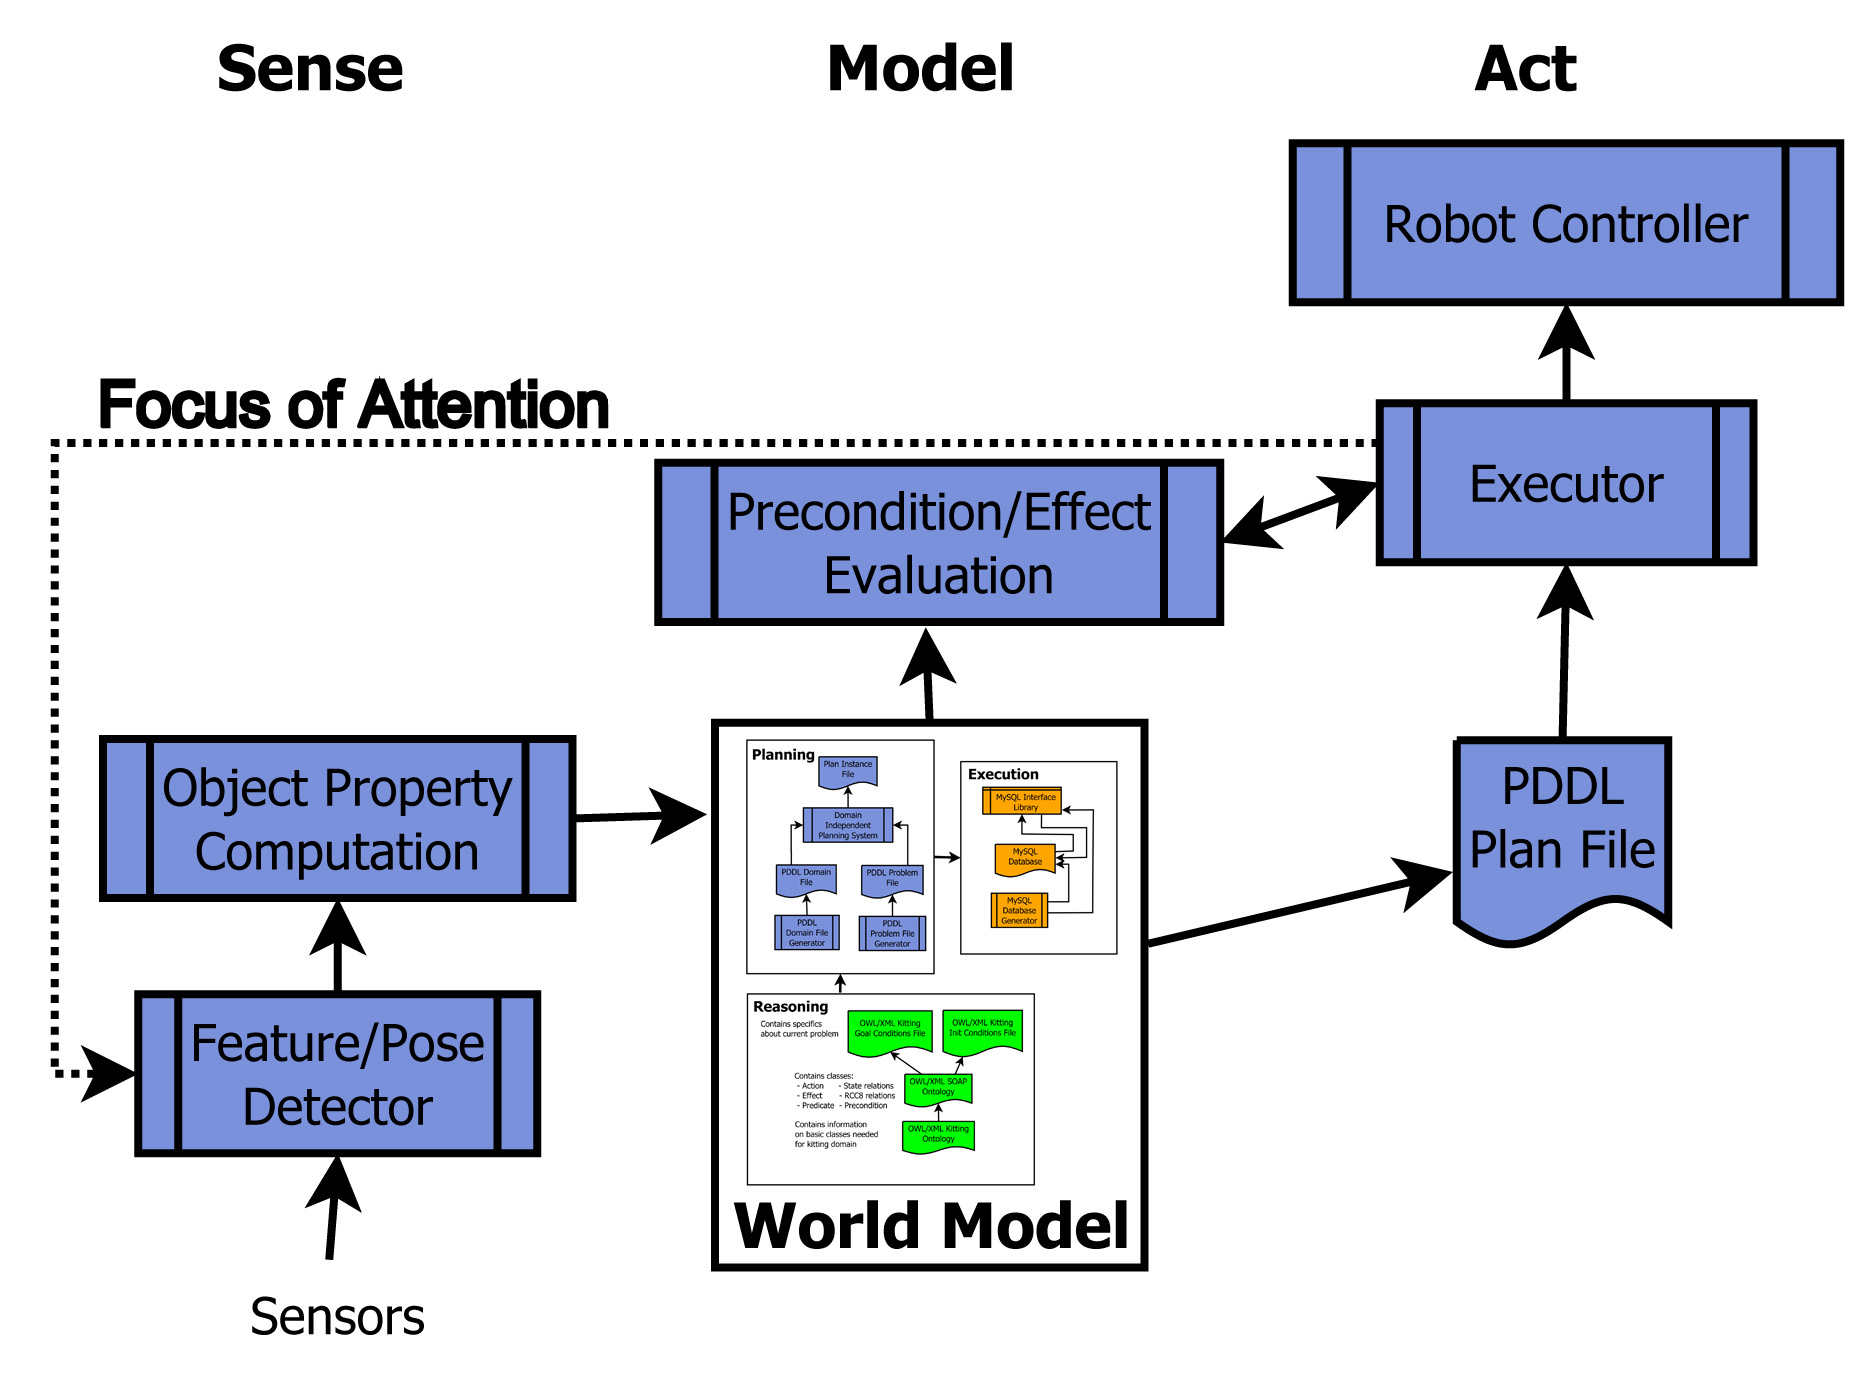
\includegraphics[width=8.5cm]{images/RITAExecution.jpg}
\caption{Major components that make up the Sense--Model--Act paradigm of the kitting station.}
\label{fig:SenseModelAct}
\end{center}
\end{figure}
\section*{BACKGROUND}
In order to experiment with robotic systems, a researcher requires a controllable robotic platform, a control system that interfaces to the robotic system and provides behaviors for the robot to carry out, and an environment to operate in.  This paper examines an open source (the game engine is free, but license restrictions do apply), freely available framework capable of fulfilling all of these requirements. This framework is composed of the USARSim framework that provides the robotic platform and environment, and the ROS framework that provides the control system.

\subsection*{The USARSim Framework}
USARSim~\cite{CARPIN.LNAI.2006,WANG.WSC.2003} is a high-fidelity physics-based simulation system based on the Unreal Developers Kit (UDK)~\cite{UDKWeb} from Epic Games. USARSim was originally developed under a National Science Foundation grant to study Robot, Agent, Person Teams in Urban Search and Rescue~\cite{LEWIS.ICHC.2003}. Since that time, it has been turned into a National Institute of Standards and Technology (NIST)-led, community-supported open source project that provides validated models of robots, sensors, and environments.

%Altogether, the Karma Physics engine~\cite{KarmEngine} and high-quality 3D rendering facilities of the Unreal game engine allow the creation of realistic simulation environments that provide the embodiment of a robotic system. Furthermore, USARSim comes with tools to develop objects and environments (Unreal Editor) and it is possible to control actors in the game through a TCP/IP socket API.

Through its usage of UDK, USARSim utilizes the physX physics engine~\cite{physXWeb} and high-quality 3D rendering facilities to create a realistic simulation environment that provides the embodiment of, and the environment for a robotic
system. The current release of USARSim consists of various model environments, models of commercial and experimental robots, and sensor models. High fidelity at low cost is made possible by building the simulation on top of a game engine. By delegating  simulation specific tasks to a high volume commercial platform (available for free to most users) which provides superior visual rendering and physical modeling, full user effort can be devoted to the robotics-specific tasks of modeling platforms, control systems, sensors, interface tools and environments. These tasks are in turn accelerated by the advanced editing and development tools integrated with the game engine. This leads to a virtuous spiral in which a wide range of platforms can be modeled with greater fidelity in a short period of time.

USARSim was originally based upon simulated environments in the USAR domain. Realistic disaster scenarios as well as robot test methods were created (Figure~\ref{TestRoom}).
Since then, USARSim has been used worldwide and more environments have been developed for different purposes. Other environments such as the NIST campus (Figure~\ref{3D_World-b}) and factories (Figure~\ref{3D_World-c}) have been used to test the performance of algorithms in different efforts~\cite{WANG.HFES.2005,BALAGUER.IROS.2008,KOOTBALLY.ITEA.2010}. The simulation is also widely used for the RoboCup Virtual Robot Rescue Competition \cite{RoboCupWeb}, the IEEE Virtual Manufacturing and Automation Challenge \cite{VMACWeb}, and has been applied to the DARPA Urban Challenge (Figure~\ref{3D_World-a}).

\begin{figure}[t!]
\centering
\subfigure[Test Room.]{\label{TestRoom}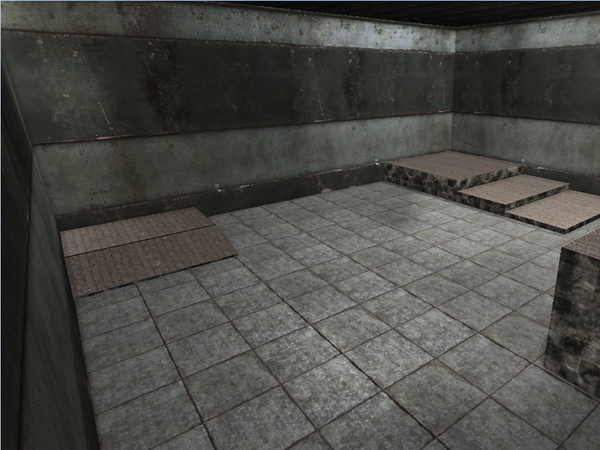
\includegraphics[width=4cm]{Figures/Worlds/testRoom.jpg}}\qquad
\subfigure[NIST main
campus.]{\label{3D_World-b}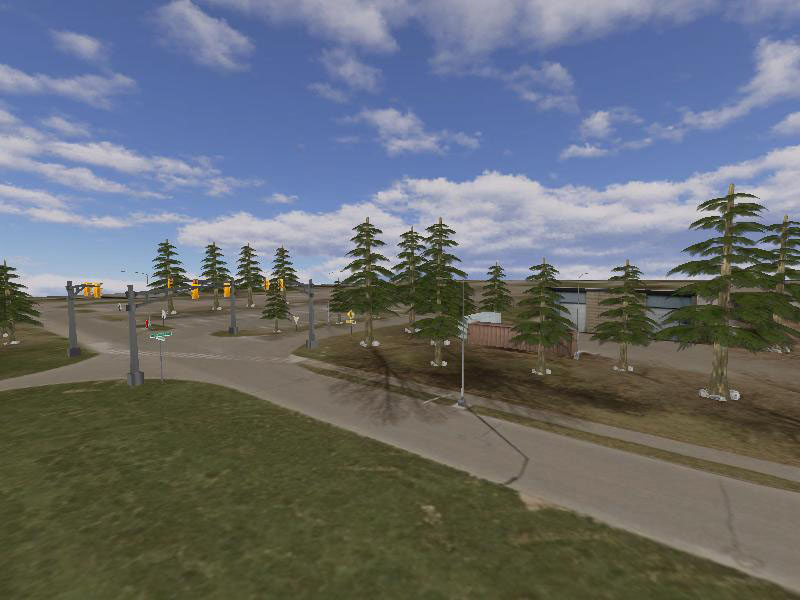
\psfig{file=Figures/Worlds/nist2.jpg,width=4cm}}\qquad
\subfigure[Factory,]{\label{3D_World-c}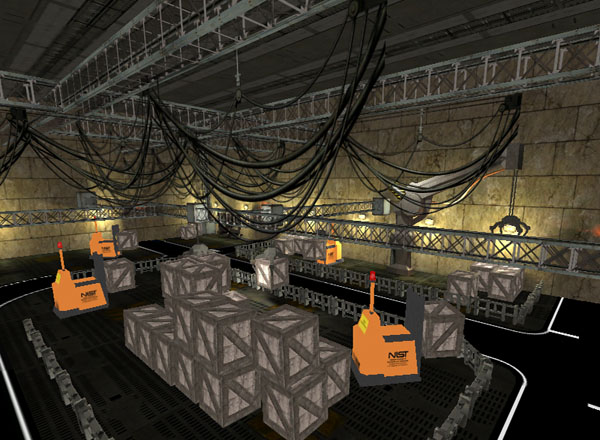
\psfig{file=Figures/Worlds/factory.jpg,width=4cm}}\qquad%
\subfigure[Road course.]{\label{3D_World-a}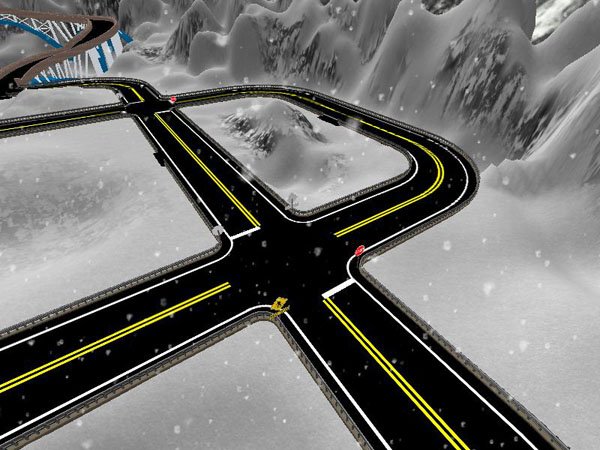
\psfig{file=Figures/Worlds/arda1.jpg,width=4cm}}
\caption{Sample of 3D environments in USARSim.} \label{3D_World}
\end{figure}

USARSim was initially developed with a focus on differential drive wheeled robots. However, USARSim's open source framework has encouraged wide community interest and support that now allows USARSim to offer multiple robots, including humanoid robots (Figure~\ref{Fig:Nao}), aerial platforms (Figure~\ref{Fig:AirRobot}), robotic arms (Figure~\ref{Fig:KR60}), and commercial vehicles (Figure~\ref{Fig:Kiva}). In USARSim, robots are based on physical computer aided design (CAD) models of the real
robots and are implemented by specialization of specific existing classes. This structure allows for easier development of new platforms that model custom designs.

All robots in USARSim have a chassis, and may contain multiple wheels, sensors, and
actuators. The robots are configurable (e.g. specify types of
sensors/end effectors) through a configuration file that is read at run-time. The properties of the robots can
also be configured, such as the battery life and the frequency of
data transmission.

\begin{figure}[t!]
\centering
\subfigure[Aldebaran Robotics Nao.]{\label{Fig:Nao}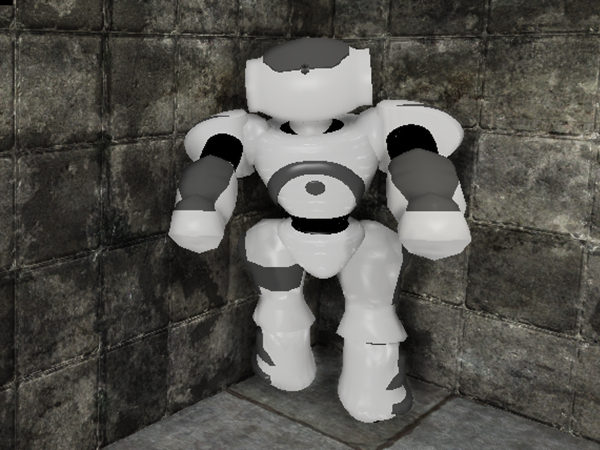
\includegraphics[width=4cm]{Figures/Robots/nao.jpg}}\qquad
\subfigure[Air Robot AR100B.]{\label{Fig:AirRobot}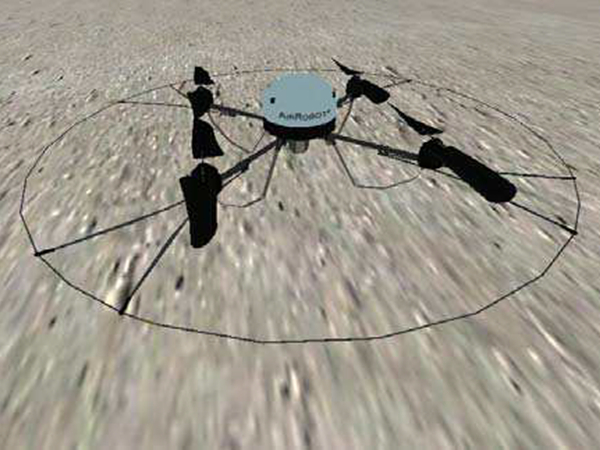
\includegraphics[width=4cm]{Figures/Robots/airRobot_2.jpg}}\qquad
\subfigure[Kuka KR60,]{\label{Fig:KR60}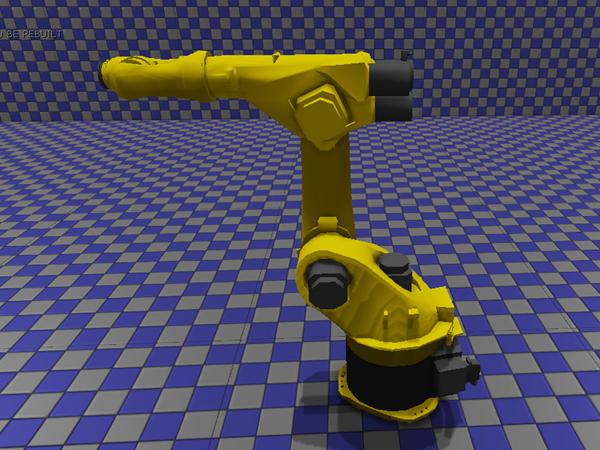
\includegraphics[width=4cm]{Figures/Robots/kr60.jpg}}\qquad
\subfigure[Kiva Robot.]{\label{Fig:Kiva}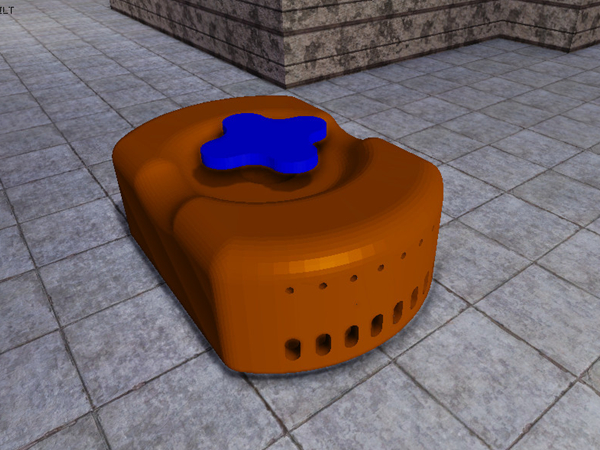
\includegraphics[width=4cm]{Figures/Robots/kiva.jpg}}
\caption{Sample of vehicles in USARSim.}
\end{figure}

\subsection*{The ROS Framework}
ROS~\cite{ROSWeb} is an open source framework designed to provide an abstraction layer to complex robotic hardware and software configurations. It provides libraries and tools to help software developers create robot applications and has found wide use in both industry and academia. Examples of ROS applications include
Willow Garage's Personal Robots Program~\cite{WYOBEK.ICRA.2008} and the Stanford University STAIR project~\cite{QUIGLEY.AAAI.2007}. Developers of ROS code are encouraged to
contribute their code back to the community and to provide documentation and maintenance of their algorithms.

ROS possesses a large range of tools and services that both users and developers alike can benefit from. The philosophical goals of ROS include an advanced set of criteria and can be summarized as: peer-to-peer, tools-based, multi-lingual, thin, and free and open-source~\cite{QUIGLEY.ICRA.2009}. Furthermore, debugging at all levels of the software is made possible with the full source code of ROS being publicly available. Thus, the main developers of a project can benefit from the community and vice-versa.

\subsubsection*{Nomenclature}
ROS uses the concept of nodes, messages, topics, services, stacks, and packages. These terms are used throughout the rest of the paper and are detailed below~\cite{QUIGLEY.ICRA.2009}.
\begin{itemize}
\item[-] Node: A process that performs computation. Nodes communicate with each other by passing messages.
\item[-] Message: A strictly typed data structure. A node sends a message by publishing it to a given topic.
\item[-] Topic: A communication channel between two or more
nodes. A node that is interested in a certain kind of data will subscribe
to the appropriate topic. There may be multiple concurrent
publishers and subscribers for a single topic, and a single
node may publish and/or subscribe to multiple topics.
\item[-] Service: A remote procedure call defined by a string name and a pair
of strictly typed messages: one for the request and one for
the response.
\item[-] Package: A compilation of nodes that can easily be compiled and ported to other computers. Packages are necessary to build a complete ROS-based robot control system.
\item[-] Stack: Packages in ROS are organized into ROS stacks which simplifies the process of code sharing. 

\end{itemize} 

\section*{THE USARSIM/ROS INTERFACE}\label{s:interface}
USARSim is designed to communicate over an American Standard Code for Information Interchange (ASCII) Transmission Control Protocol/Internet Protocol (TCP/IP) socket with a host computer. The host computer initiates the socket interface and ``spawns'' the desired robot into the simulated world that is currently running on the game server. A robot's configuration is controlled by an initialization file that resides on the simulation system's computer. This file controls such aspects as sensor configuration, battery life, and simulated noise models. Please see the USARSim wiki for more information on robot configuration~\cite{USARSimWeb}.  One socket connection is established per simulated robot, with both commands and sensor data being transmitted over the socket. An additional separate socket is established for high-volume sensors such as camera systems.

ROS stacks are designed to ``bottom out'' at a hardware abstraction layer that provides basic topics to and from the robot. For example, the mobility stack expects to control a platform by writing commands to low-level topics that control items such as platform velocities, and to receive feedback from sensors over other low-level topics. These stacks may also place constraints or naming conventions on the topics.  In order to close this low-level loop between ROS and USARSim, a USARSim package was created. This package contains a node called {\it RosSim} that publishes a ROS transform tree (from the ROS {\it tf} package) and sensor messages, and also accepts platform and actuator motion commands. When run, it provides a mechanism for spawning a robot in USARSim, and then auto-discovering the robot's sensors, actuators, and drive configuration in order to provide the necessary ROS topics. 
 \begin{table}[t!]
    \begin{center}
    \small{
    \begin{tabular}{ | l | l | p{4cm} |}
    \hline
    Parameter & Default & Definition \\ \hline
   robotType & P3AT & Type of robot to spawn. \\ \hline
   hostname & localhost & Name of host running USARSim. \\ \hline
   port & 3000 & TCP/IP Port on which USARSim listens. \\ \hline
   startPosition & Vehicle1 & Named location where robot should be spawned. This location is simulated world dependent. \\ \hline
   odomSensor & InsTest & Odometry sensor that should be used as the default sensor for feeding the {\it odom} topic of ROS.\\ \hline
    \end{tabular}
   }
    \caption{Parameters for USARSim ROS node.}
    \label{Table:USARSimNode}
    \end{center}
\end{table}
\begin{figure}[t!]
\centering
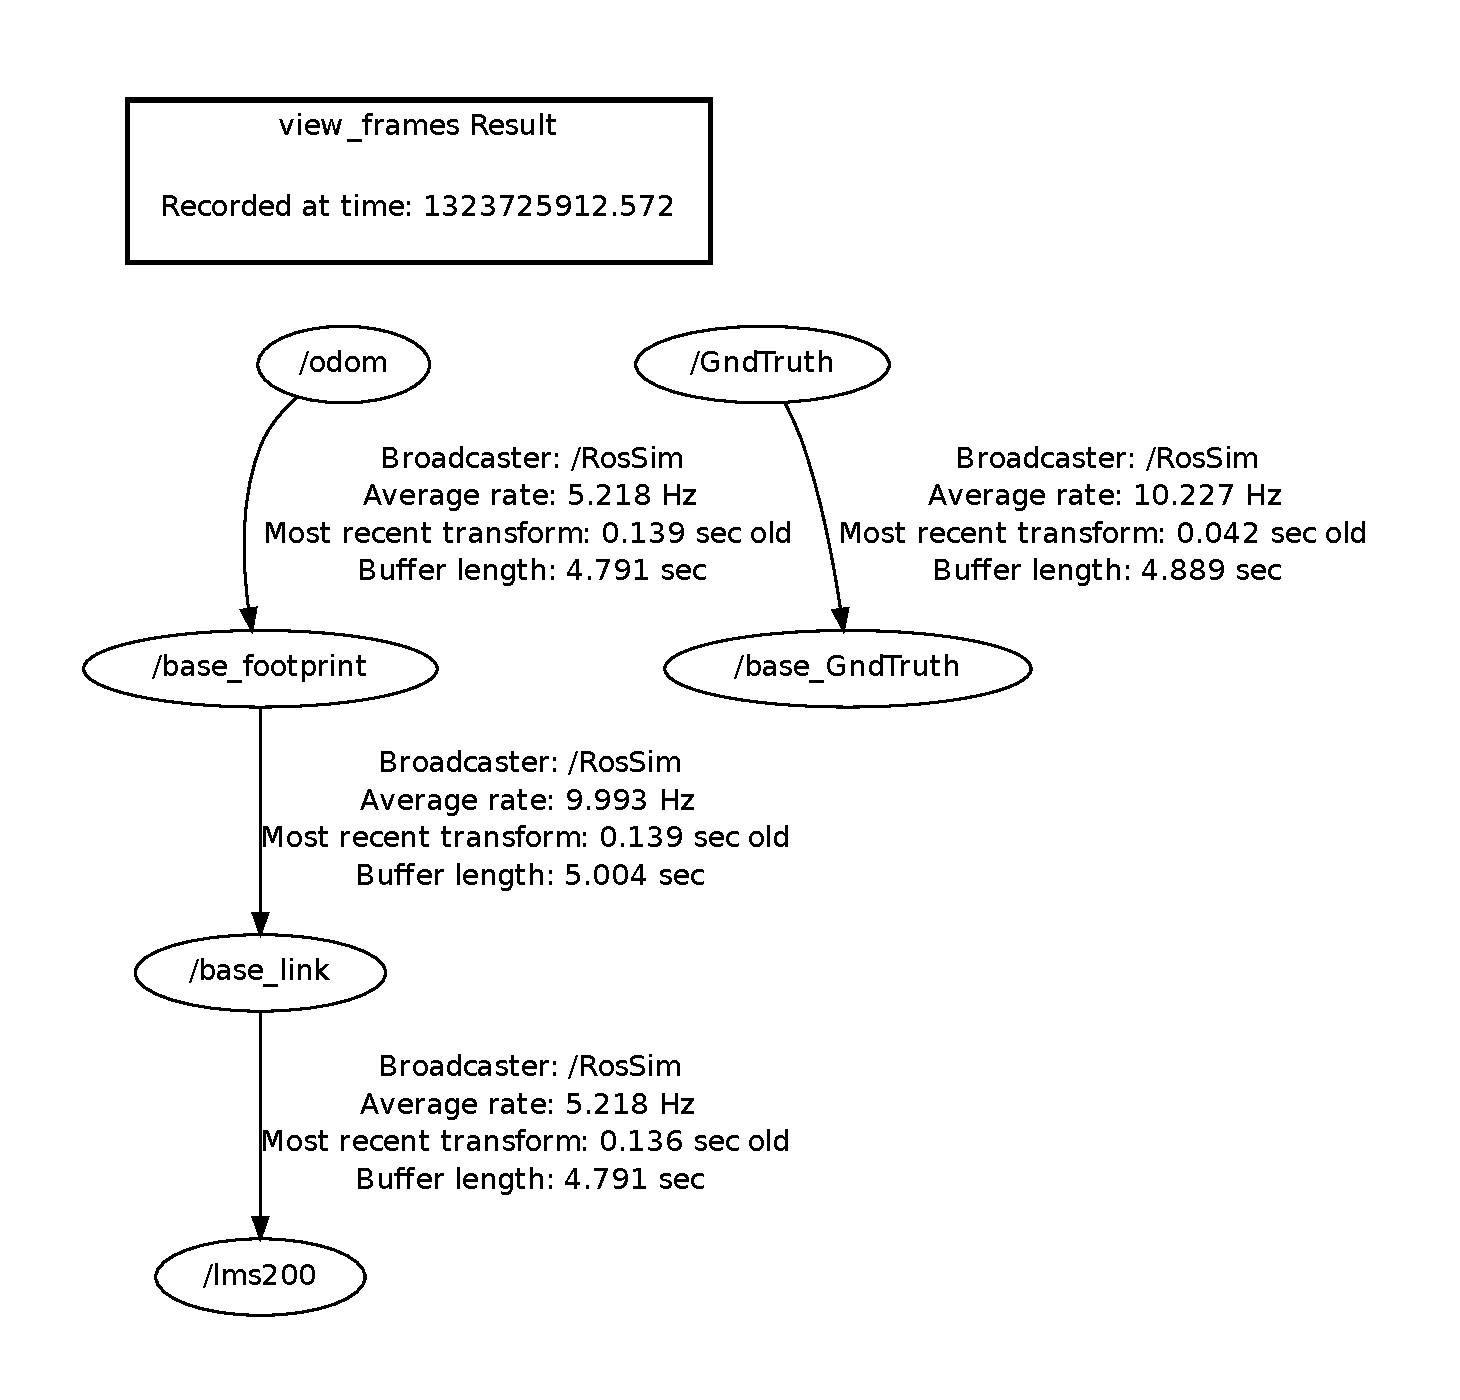
\includegraphics[width=8cm]{Figures/ROS/P3ATFrames.pdf}
\caption{Auto-generated tf Transform tree for P3AT robot.}
\label{Fig:P3ATTransformTree}
\end{figure}

The {\it RosSim} node relies on several parameters for its configuration. These are detailed in Table~\ref{Table:USARSimNode}, and provide information necessary for the creation of a robot in USARSim and a transform tree in ROS. A transform tree for the P3AT robot is shown in Figure~\ref{Fig:P3ATTransformTree}. This transform tree is built automatically from data obtained from the USARSim {\it geo} and {\it conf} messages. Since USARSim supports more than one localization sensor on a robot, the {\it odomSensor} parameter is consulted to determine which sensor should be built into the tree. That sensor's name is automatically changed to {\it odom}. The {\it base\_footprint}, representing the robot platform and the {\it base\_link}, representing robot sensor mounting points, are also automatically generated. Additional localization sensors (e.g., the ground truth sensor for the P3AT robot) are provided with their own transform tree.

Vehicle movement commands into USARSim vary depending on the robot type. For example, skid-steered vehicles require left and right wheel velocities while Ackerman steered vehicles required steering angle and linear velocity. ROS provides a {\it cmd\_vel} topic that includes both linear and angular velocities. The {\it RosSim} node automatically converts these velocities into the appropriate commands and values for the USARSim simulator based on the robots steering type, wheelbase, and wheel separation. Vehicle speeds are also clamped to not exceed maximum velocities that are set in the simulation.

\subsection*{Sensor Interface} 
ROS provides a rich vocabulary of sensor interface messages. The {\it RosSim} node strives to automatically match simulated sensors to the appropriate ROS topic. Currently, USARSim's inertial navigation, ground truth, and LADAR sensors are supported. These sensors automatically join the robot transform tree and publish their sensor messages at the rate that the {\it RosSim} node receives the sensor output. It is the intent of the authors to implement the full array of USARSim's sensors as time and resources permit.

The ROS/USARSim interface allows one to utilize known, published algorithms with simulated sensors and environments. However, the computational expense of the sensor processing must still be carried by the target hardware. One benefit of simulation is that one can not only simulate raw sensor output, but also the results from complex sensor processing tasks. One such example is the USARSim object recognition sensor. This sensor  is simulated in much the same manner as a laser scanner. However, instead of reporting the range that each beam travels, the sensor accumulates the number of beam hits that occur on each detected object. The number of hits, along with the percentage of the object that is visible may then be used to determine the amount of noise to add to the objects position and recognized type. This information may then be sent over standard ROS topics, without incurring the overhead burden of running the actual object and pose recognition algorithms.

\subsection*{Mobile Robot Control with the ROS Navigation Stack}
Control of mobile robots through the ROS/USARSim interface is performed with the ROS navigation stack~\cite{RosNavWeb}. The navigation stack provides for 2D navigation and takes in information from odometry, sensor streams, and a goal pose while outputting safe velocity commands that are sent to a mobile base. The velocity commands are sent in the form of: x velocity, y velocity, theta velocity. Better performance of the navigation stack can be achieved by meeting the following requirements:
\begin{itemize}
\item[-] The robot has to use either differential drive or holonomic drive.
\item[-] A planar laser has to be mounted on the mobile base. This laser is used for map building and localization.
\item[-] The performance of the navigation stack will be best on robots that are nearly square or circular. It does work on robots of arbitrary shapes and sizes, but it may have difficulty with large rectangular robots in narrow spaces like doorways.
\end{itemize}

Although different models of mobile robot are developed in USARSim, the Pioneer 3-AT (P3AT) (Figure~\ref{fig:p3at}) appears to be a suitable candidate to use the navigation stack. The P3AT is a small square-shaped differential drive wheeled robot. As configured in our experiments, it includes a SICK Laser Measurement Sensor (LMS) 200 mounted on his base. The P3AT is also widely employed for research and prototyping applications involving mapping, navigation, monitoring, reconnaissance, vision, manipulation, cooperation, and other behaviors.

\begin{figure}[t!]
\centering
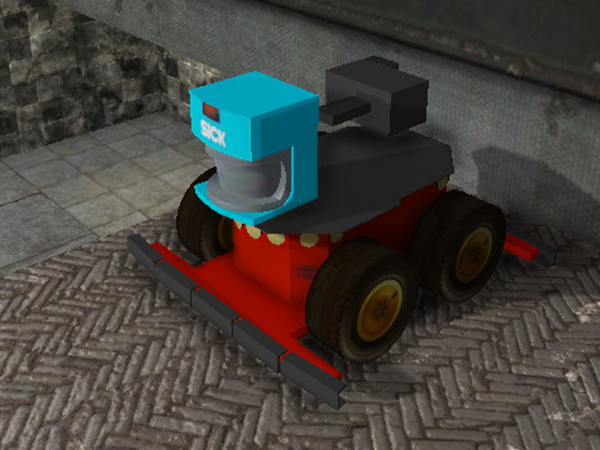
\includegraphics[width=4cm]{Figures/Robots/p3at.jpg}
\caption{Pioneer 3-AT (P3AT) in USARSim.}\label{fig:p3at}
\end{figure}




\subsubsection*{Low-level Navigation}
The ROS/USARSim interface allows the start-up and the control of the default P3AT base controllers by directly sending velocity commands to the base. This task was performed using the following commands:
\begin{enumerate}
\item\footnotesize{Bring up an environment in USARSim.        }
\item\footnotesize{\$roscore}
\item\footnotesize{\$roslaunch usarsim usarsim.launch}
\item\footnotesize{\$rosrun teleop\_twist\_keyboard teleop\_twist\_keyboard.py}
\item\footnotesize{\$rosrun gmapping slam\_gmapping scan:=lms200 \_odom\_frame:=odom}
\end{enumerate}

In step 1. an environment is started on the server side (USARSim). If an environment is not up and running, passing messages between ROS and USARSim will fail. Step 2. starts {\it roscore}, a collection of nodes and programs that are a pre-requisites of a ROS-based system for ROS nodes to communicate. Step 3. launches the {\it usarsim.launch} file. This launch file contains the parameters specified in Table~\ref{Table:USARSimNode} and starts the {\it RosSim} node that provides a connection between ROS and USARSim. Step 4. starts the {\it teleop\_twist\_keyboard} node which sends velocity commands to the {\it RosSim} node through the computer keyboard. At this point, the P3AT can be controlled by keyboard teleop in the USARSim environment. Step 5. starts the node {\it slam\_gmapping} which transforms each incoming scan from the laser into the odometry tf frame to build a map. Here, the topic {\it scan} is used to create the map with the parameter {\it \_odom\_frame}, the frame attached to the odometry system.

%\begin{figure}[t!]
%\centering
%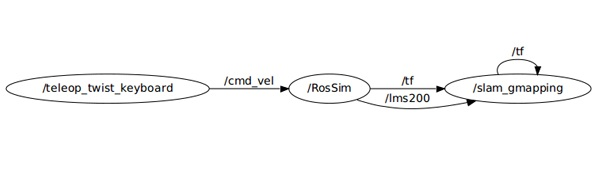
\includegraphics[width=9cm]{Figures/Misc/low-level.jpg}
%\caption{Mobile robot control using \texttt{teleop}.}\label{fig:teleop}
%\end{figure}

\begin{figure}[t!]
\centering
\resizebox{\columnwidth}{!}{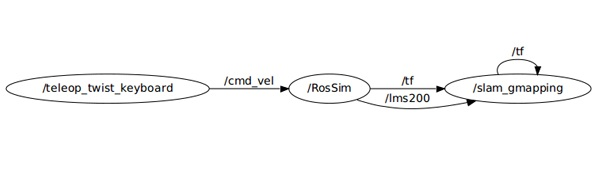
\includegraphics{Figures/Misc/low-level.jpg}}
\caption{\label{fig:teleop}Mobile robot control using {\it teleop}}
\end{figure}


Figure~\ref{fig:teleop} is a graph generated by rxgraph with the option ``quiet". The graph illustrates the communication between the nodes {\it RosSim}, {\it teleop\_twist\_keyboard}, and {\it slam\_gmapping}. The keyboard inputs are converted in velocity commands and then communicated to the {\it RosSim} node on the topic {\it cmd\_vel}. {\it slam\_gmapping} uses the topics ({\it lms200}) and ({\it tf}) as inputs to build the map. To save the generated map, the following command is used:

\begin{itemize}
\item[]\$rosrun map\_server map\_saver
\end{itemize}

\begin{figure}[t!]
\centering
\subfigure[USARSim environment.]{\label{Fig:vmac-usarsim}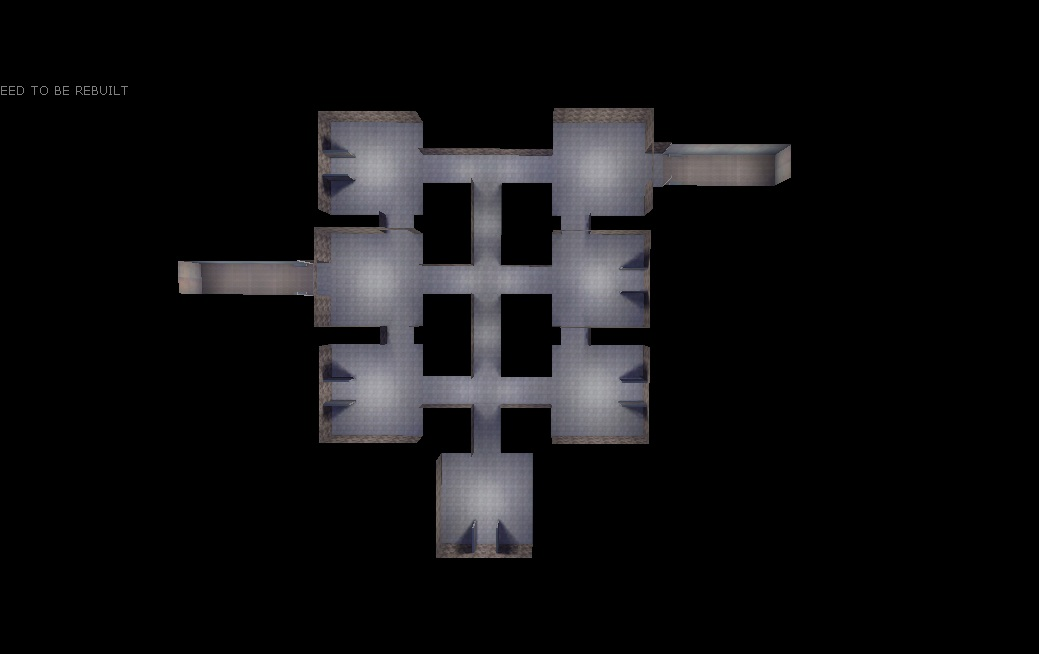
\includegraphics[width=4.1cm]{Figures/Misc/vmac-usarsim2.jpg}}\qquad
\subfigure[Map of the environment.]{\label{Fig:vmac-usarsim-map}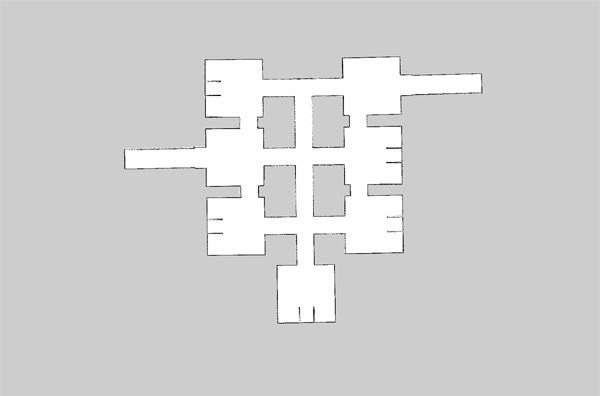
\includegraphics[width=4cm]{Figures/Misc/vmac-usarsim-map.jpg}}
\caption{Environment in USARSim and the corresponding map.}
\end{figure}
The generated map is stored in pair of files: a YAML file (YAML is recursively defined as ``YAML Ain't Markup Language'') which describes the map meta-data and the image file that encodes the occupancy data. Figure~\ref{Fig:vmac-usarsim} is a bird's eye view of the environment used to run the teleop command on the P3AT and Figure~\ref{Fig:vmac-usarsim-map} is the map generated by the {\it map\_saver} utility-command.



%\texttt{RosSim} publishes two topics for the odometry (\texttt{GndTruth} and \texttt{InsTest}), one topic to keep track of multiple coordinate frames over time \texttt{tf}, and a topic for the laser scanner (\texttt{lms200}).



\subsubsection*{High-level Navigation}
The ROS/USARSim interface also provides high-level navigation through the navigation stack. At this level, goals are sent to the P3AT to move to a particular location in the environment. Navigation at a high level is possible with the action specification for {\it move\_base}. This package provides an implementation of an action ({\it actionlib}) that, given a goal in the world, will attempt to reach it with a mobile base. The {\it move\_base} node provides a ROS interface for configuring, running, and interacting with the navigation stack on a robot. The {\it move\_base} node links together a global and local planner to accomplish its global navigation task.

%\begin{figure}[t!]
%\centering
%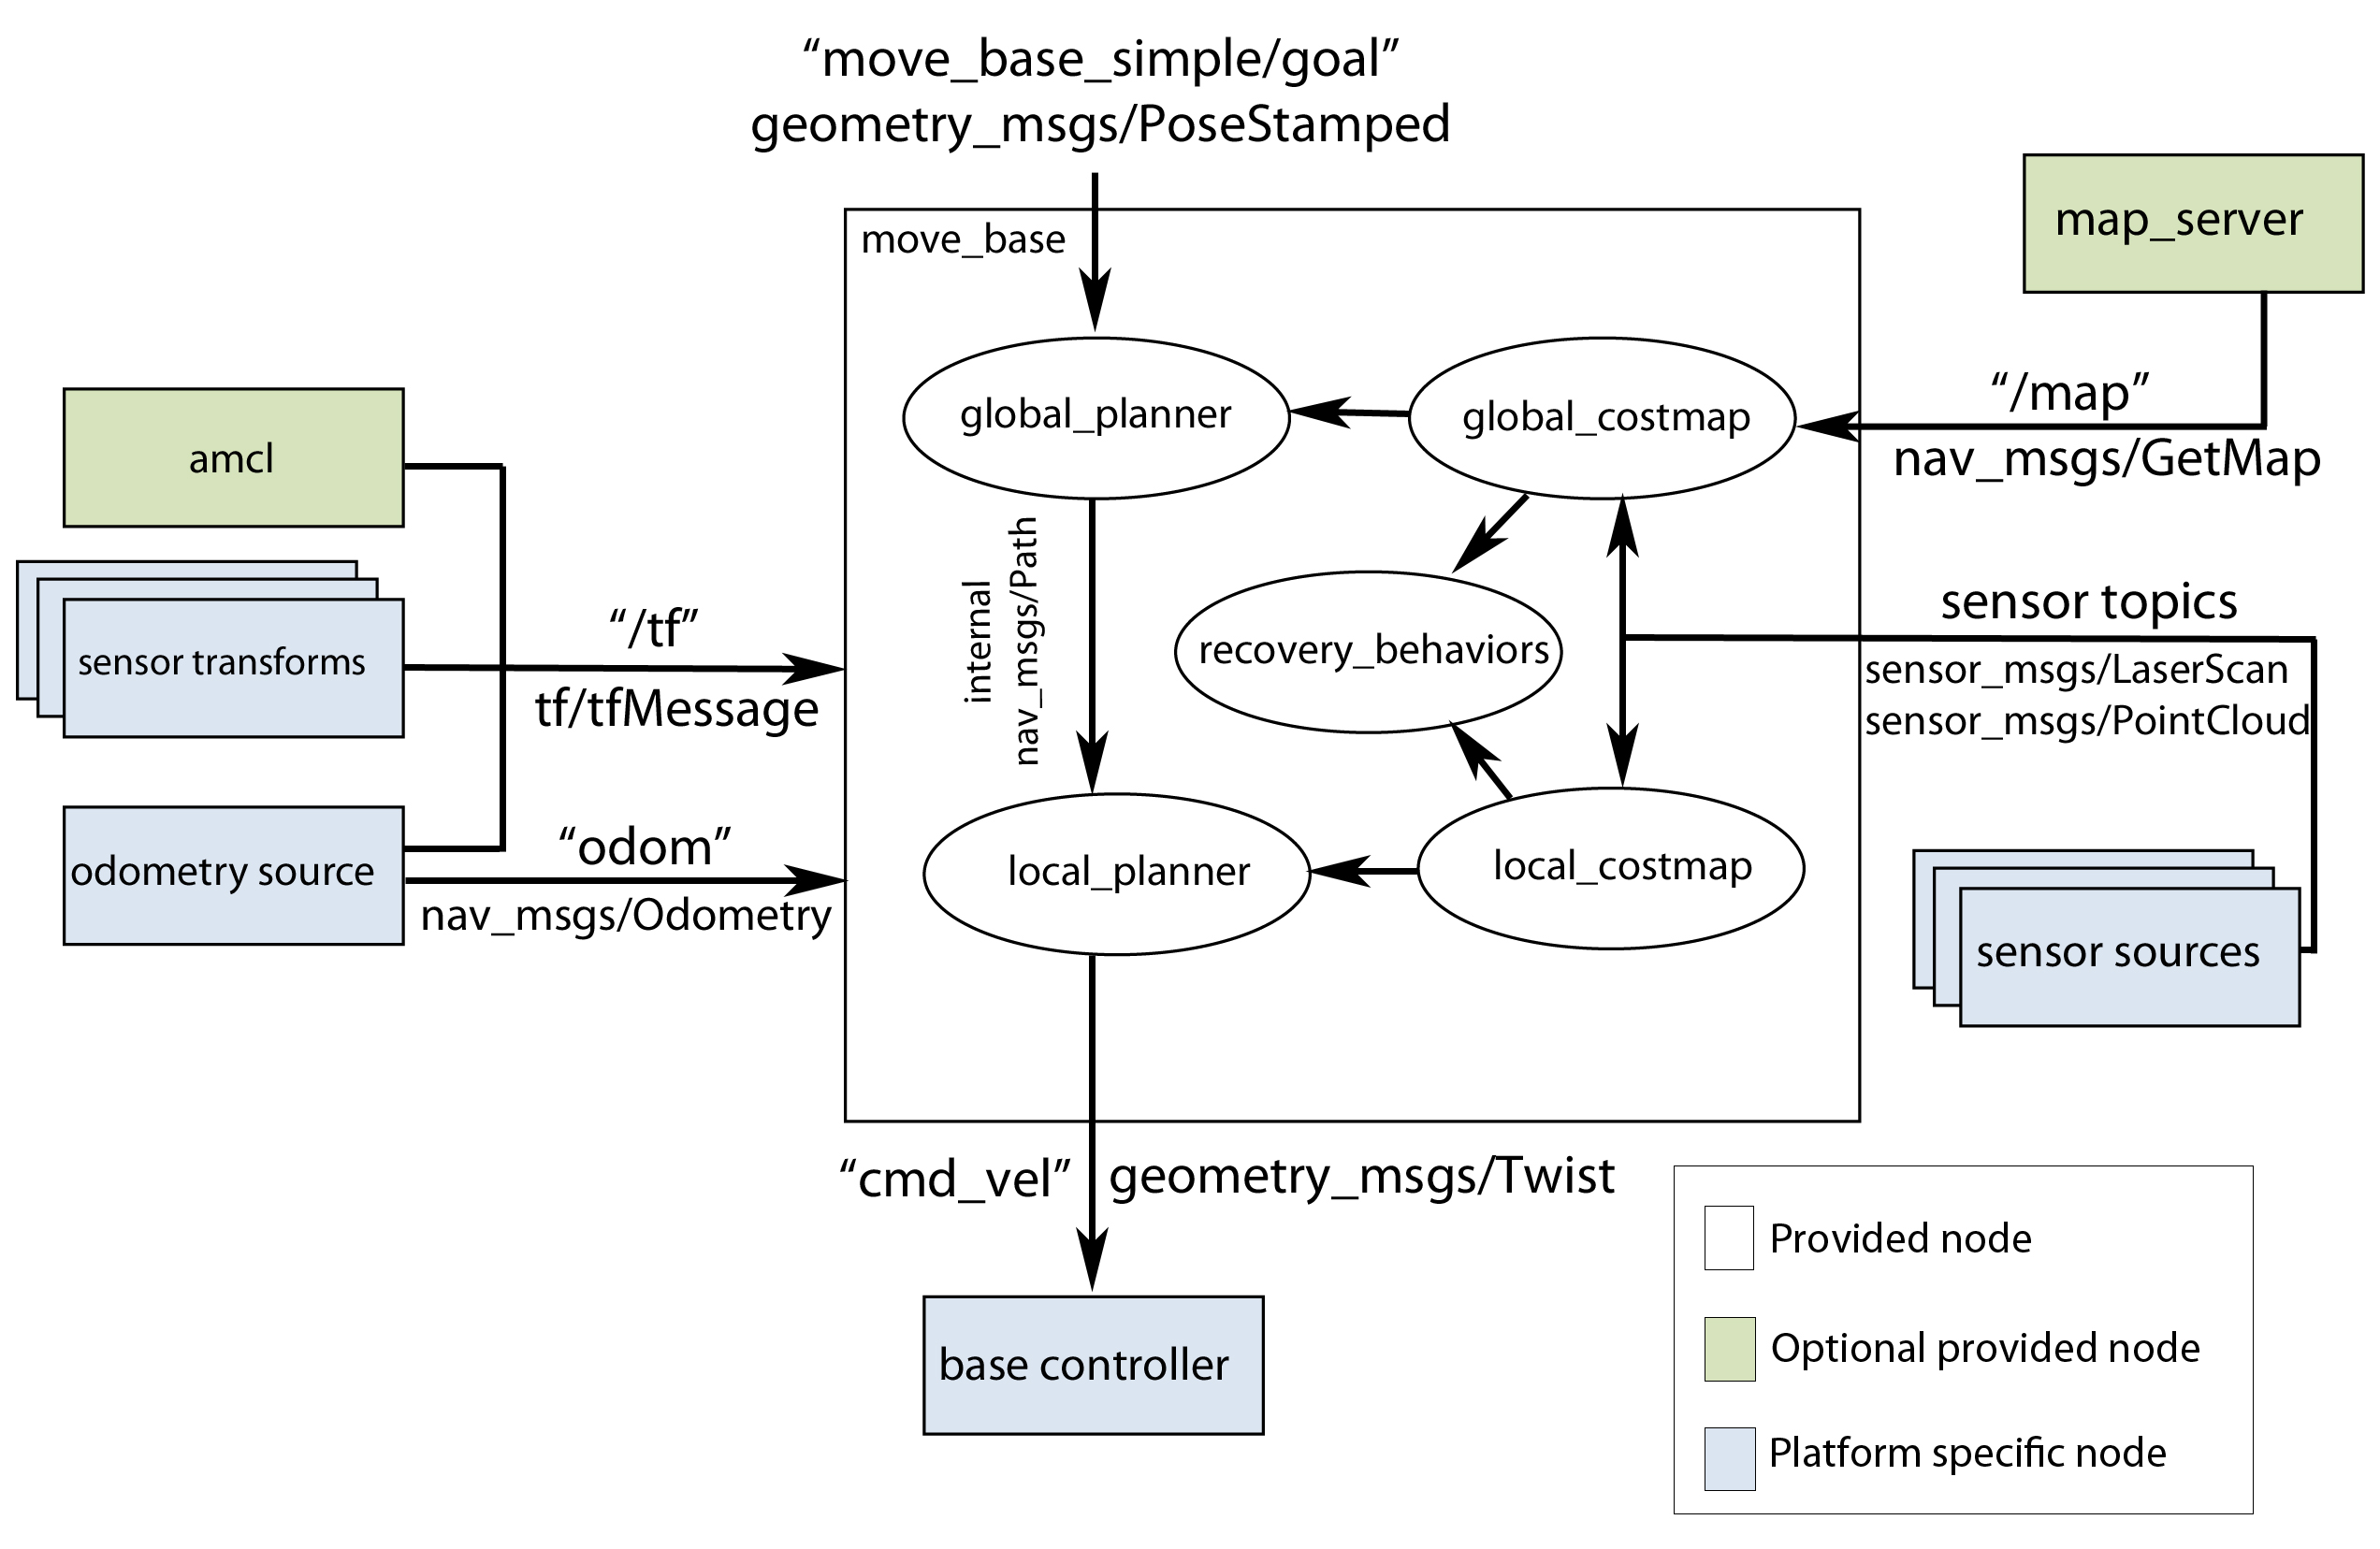
\includegraphics[width=10cm]{Figures/Misc/Navigation_Stack.jpg}
%\caption{Navigation stack setup using \texttt{move\_base}.}\label{fig:navigation_stack}
%\end{figure}


\begin{figure}[t!]
\centering
\resizebox{\columnwidth}{!}{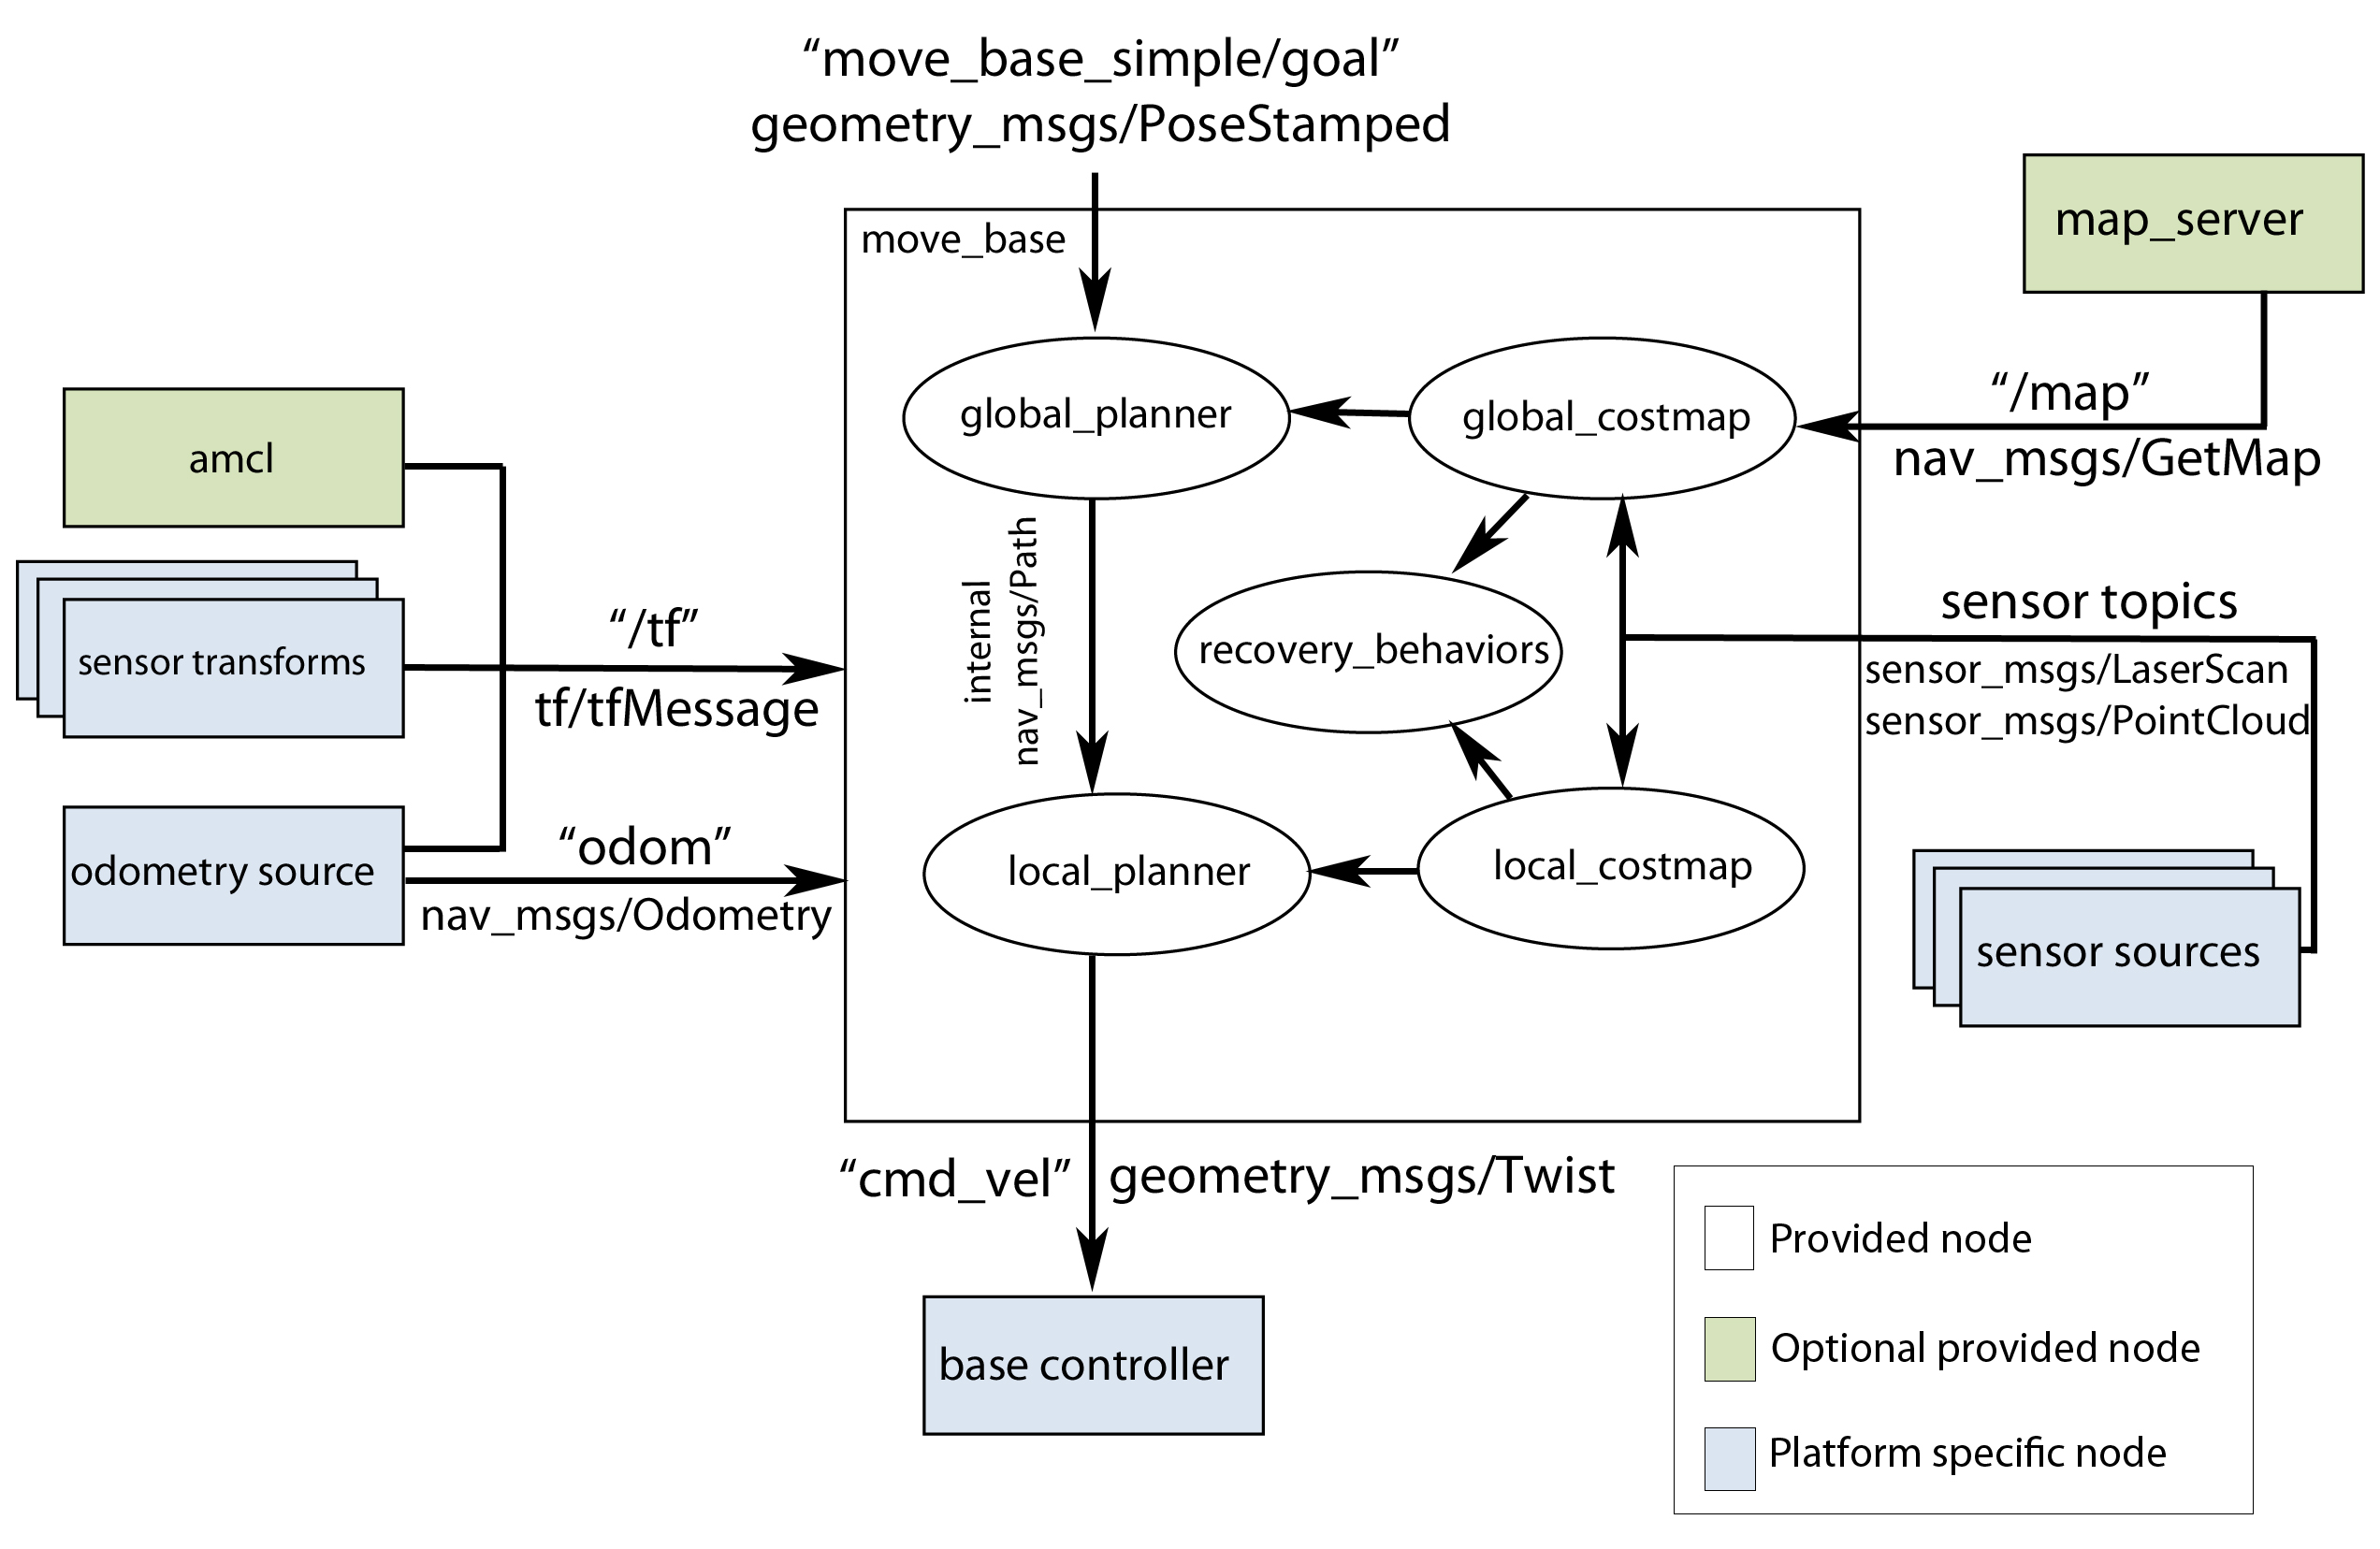
\includegraphics{Figures/Misc/Navigation_Stack.jpg}}
\caption{\label{fig:navigation_stack}Navigation stack setup using {\it move\_base}}
\end{figure}

Figure~\ref{fig:navigation_stack} (taken from~\cite{MoveBase}) depicts a high-level view of the {\it move\_base} node and its interaction with other components of the navigation stack. The white components are required components, the green components are optional components, and the blue components must be created for each robot platform. The white and green components are already implemented. For the navigation stack to work properly for the P3AT, the nodes and topics generated should match the configuration of the {\it move\_base} node with the navigation stack.


Before running the {\it move\_base} node on the P3AT, localization, mapping, and navigation information are filled in the {\it move\_base.launch} file:
\begin{itemize}
 \item [-] Localization uses map, laser data, and odometry to situate the robot in relation to the environment. The {\it amcl} and the {\it map\_server} nodes are necessary for robot localization. {\it amcl} is a probabilistic localization system for a robot moving in 2D and implements the KLD-sampling\cite{DIETER.IJRS.2003}. The {\it amcl} node is launched from the examples directory of the amcl package.
% and is included in {\it move\_base.launch} as one of its parameters.
\item [-] The {\it map\_server} node uses an {\it a priori} map generated by the {\it map\_saver} command-line utility. The example described in this paper uses the map depicted in Figure~\ref{Fig:vmac-usarsim-map} and its corresponding YAML file.
\item [-] The navigation stack uses cost-maps files (YAML files) to store information about obstacles in the world:
\begin{itemize}
\item [-] A global cost-map for creating long-term plans.
\item [-] A local cost-map for local planning and obstacle avoidance.
\item [-] A common cost-map file which stores configuration options used by the global and local cost-maps.
\end{itemize}
\item [-] The navigation stack uses a base local planner to compute velocity commands to send to the robot. Information on the base local planner is stored in a YAML file which sets configuration options based on the specs of the robot.
\end{itemize}

Once the {\it move\_base.launch} file is set up with the appropriate configuration options, the {\it move\_base} node is run with the following command:

\begin{itemize}
\item[]\$roslaunch move\_base.launch
\end{itemize}

To send commands to the P3AT, the package {\it simple\_navigation\_goals} was created (based on~\cite{SendingSimpleGoals}). The new package mainly includes the action specification for {\it move\_base}, an action client used to communicate with the action named {\it move\_base} that adheres to the MoveBaseAction interface, and a goal to send to {\it move\_base}. Sending commands through the code to the P3AT is performed by starting the executable for the {\it simple\_navigation\_goals} package:

\begin{itemize}
\item[]\$./bin/simple\_navigation\_goals
\end{itemize}

%\begin{figure}[h!]
%\centering
%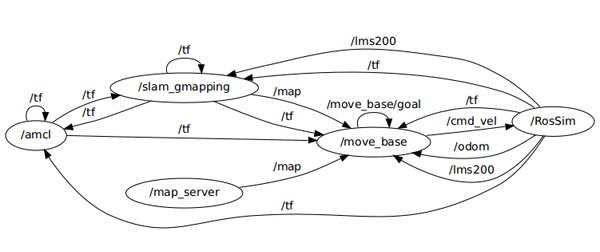
\includegraphics[width=10cm]{Figures/Misc/move_base.jpg}
%\caption{Mobile robot control with move\_base.}\label{fig:movebase}
%\end{figure}

\begin{figure}[t!]
\centering
\resizebox{\columnwidth}{!}{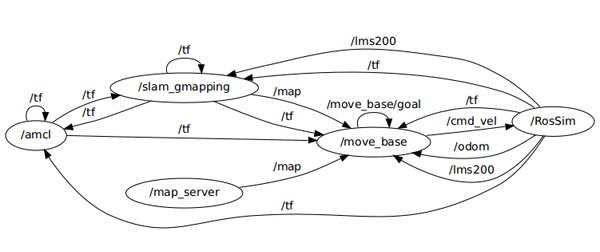
\includegraphics{Figures/Misc/move_base.jpg}}
\caption{\label{fig:movebase}Mobile robot control with {\it move\_base}.}
\end{figure}
      


Figure~\ref{fig:movebase} is a graph generated by rxgraph with the option ``quiet". The graph depicts the nodes and topics involved while sending a goal to  the navigation stack to move the P3AT. A parallel comparison of this graph with the navigation stack setup diagram (Figure~\ref{fig:navigation_stack}) reveals that the blue components have been implemented and the grey components were properly used. The node {\it move\_base} receives messages on the topic {\it tf} from the nodes {\it amcl}, {\it RosSim}, and {\it slam\_mapping}. {\it RosSim} publishes Odometry ({\it odom}) and sensor information ({\it lms200}) to {\it move\_base}. The optional node {\it map\_server} publishes the topic {\it map} to {\it move\_base}. Incoming messages are interpreted by {\it move\_base} which outputs velocity commands on the topic {\it cmd\_vel} to be sent to the node {\it RosSim}.

\subsection*{Robotic Arm Interface}
Although not as complete at the navigation interface, an interface has also been developed to allow for the use of the ROS arm\_navigation~\cite{RosArmNavWeb} stack. The {\it RosSim} node once again strives to allow for auto-discovery of the robot and thus eliminate the need for hand-generated configuration files. In the case of the arm\_navigation stack, a Unified Robot Description Format (URDF) file that describes the arm must be created as well as various launch files. 

Under USARSim, a robotic arm is composed of individual static meshes are are attached to one another via  links knows as {\it actuators}. Each actuator has its own coordinate frame. Figure~\ref{Fig:KR60Anotated} depicts a Kuka KR60 robot that has been modeled in USARSim. The position and orientation of each actuator's coordinate frame is controled by convention. Actuators must rotate (rotatory joints) or expand (prismatic joints) about the z-axis. The x-axis must point towards the next joint in the kinematic chain. The location of the axis origin is constrained such that rotation/expansion occurs around $z=0$ and the x-axis passes through the origin of the next frame in the kinematic chain. The {\it RosSim} node automatically builds the transform tree for the various actuator coordinate frames by reading the USARSim {\it Conf} and {\it Geo} messages. The transform tree for the KR60 robot is depicted in Figure~\ref{Fig:KR60TF}. This transform is published and made available to any other ROS node.

When a new robotic arm is used for the first time, the {\it usar\_urdf} node of the {\it USARSim} ROS package must be run. This node accepts the same parameters shown in Table~\ref{Table:USARSimNode} in oder to determine the robot to be created and then performs the following actions:
\begin{enumerate}
\item The node spawns the robot model inside the simulated world in order to be able to read the USARSim  {\it Conf} and {\it Geo} messages.
\item From these messages, the node composes the transform tree with a transform for each joint in the robotic arm. Information on maximum and minumum rotations of joints and maximum joint velocities and torques is also maintained.
\item The node auto-generates an URDF file that contains all of the joint and link information that defines the robot arm. Rather than exact depictions of the robot's visual form, the URDF file contains simple cylinders to represent each link.
\end{enumerate}

\begin{figure}[t!]
\centering
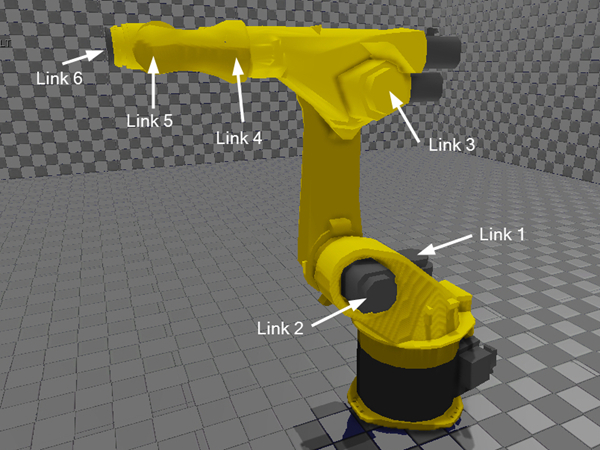
\includegraphics[width=8cm]{Figures/Robots/KR60Profile.jpg}
\caption{Location of joint axes in USARSim model of Kuka KR60 6 degree-of-freedom robot arm as depicted in USARSim.}
\label{Fig:KR60Anotated}
\end{figure}

\begin{figure}[t!]
\centering
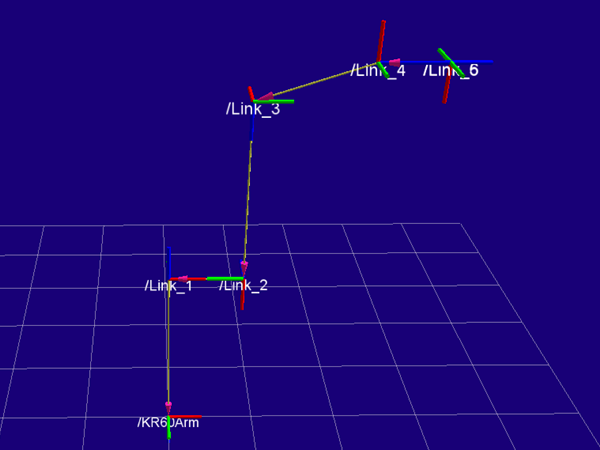
\includegraphics[width=8cm]{Figures/ROS/rviz1.png}
\caption{Depiction of joint axes from TF topic in ROS for 6 degree-of-freedom Kuka KR60 robot arm.}
\label{Fig:KR60TF}
\end{figure}

This URDF file may now be utilized by the arm\_naviation's {\it Planning Description Configuration Wizard} in order to generate a stack that contains specific launch files that will be used in arm planning.





%\section*{SETUP AND RUN THE INTERFACE}\label{s:interface}

\section*{CONCLUSION AND FUTURE WORK}\label{s:conclusion}
This paper has presented a new ROS package that allows for the seemless interface of USARSim with ROS. The package provides for auto-discovery of robots and sensors, and produces the standard ROS topics that one would expect from a physical platform. Further work is still required to auto-generate ROS launch files for running standard motion control algorithms for both platform and arm control. In addition, additional sensors must have their USARSim interfaces wrapped to be supported in the ROS environment.


%%%%%%%%%%%%%%%%%%%%%%%%%%%%%%%%%%%%%%%%%%%%%%%%%%%%%%%%%%%%%%%%%%%%%%
% The bibliography is stored in an external database file
% in the BibTeX format (file_name.bib).  The bibliography is
% created by the following command and it will appear in this
% position in the document. You may, of course, create your
% own bibliography by using thebibliography environment as in
%
% \begin{thebibliography}{12}
% ...
% \bibitem{itemreference} D. E. Knudsen.
% {\em 1966 World Bnus Almanac.}
% {Permafrost Press, Novosibirsk.}
% ...
% \end{thebibliography}

% Here's where you specify the bibliography database file.
% The full file name of the bibliography database for this
% article is asme2e.bib. The name for your database is up
% to you.
\bibliographystyle{asmems4}
\bibliography{PMAS-asme}



\end{document}
